
In this section we will introduce \csim by means of a simple example.
We will use \csim to simulate a model where a
\secref{classLifNeuron}{leaky-integrate-and-fire} neuron (LIF neuron)
is driven by a Poisson spike train which is transmitted by a
\secref{classDynamicSpikingSynapse}{dynamic synapse}.

\begin{center}
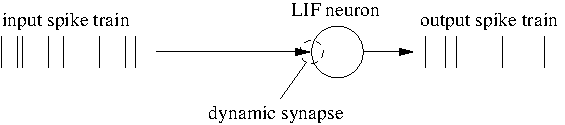
\includegraphics{first-model}
\end{center}

%\Subsection{Setting up the simulation}{subsec:setup}

\subsection{Creating Objects}

Each element/entity of the simple model we will implement, will be
simulated by a corresponding \emph{object} in \csim. The following
table shows the correspondence between the elements of the model and
the \emph{class} of the object used to simulate the element
%
\begin{center}
\begin{tabular}{l|l}
\textbf{element of model} & \textbf{class of \csim object} \\\hline
input spike train & \texttt{SpikingInputNeuron} \\
dynamic synapse & \texttt{DynamicSpikingSynapse} \\
LIF neuron & \texttt{LifNeuron}
\end{tabular}
\end{center}
%
Hence, for the simulation to run one must \secref{cmd:create}{create
  objects} of the given class:
%
\begin{tabbing}
\quad\tt>> i=csim('create','SpikingInputNeuron'); \\
\quad\tt>> s=csim('create','DynamicSpikingSynapse'); \\
\quad\tt>> n=csim('create','LifNeuron');
\end{tabbing}
%

\subsection{Object Handles}

The values \texttt{i, s}, and \texttt{n} returned by these
\secref{cmd:create}{create commands} are the \emph{indices} or
\emph{handles} to the created objects. The handles are the only means
to further access or modify existing objects.

\subsection{Setting Fields or Parameters}

Each of the created objects has several \emph{fields} which usually
correspond to a parameter of the model which is implemented by the
class of the object. To display for example all
\secref{classLifNeuron}{fields of the \texttt{LifNeuron}} object we
can use the command
%
\begin{tabbing}
\quad\tt>> csim('\hyperlink{cmd:get}{get}',n);
\end{tabbing}
%
This will yield the following output
%
\begin{verbatim}
  0 : LifNeuron
          Cm = 3e-08 (F)
          Rm = 1e+06 (Ohm)
    Vresting = -0.06 (V)
      Vreset = -0.06 (V)
       Vinit = -0.06 (V)
    Trefract = 0.003 (sec)
      Inoise = 0 (A)
     Iinject = 0 (A)
     Vthresh = -0.045 (V)
          Vm : 0 (V)
        type = 0
     nSpikes : 0
   nIncoming : 0
   nOutgoing : 0
\end{verbatim}
%
Some of the fields are parameters of the model (\texttt{Cm},
\texttt{Rm}, ...) which can be modified (denoted by the \texttt{'='})
others are internal state variables (\texttt{Vm} in this case) which
can not be changed (denoted by the \texttt{':'}) and yet other provide
auxiliary information (\texttt{nSpikes}, \texttt{nIncoming}, ...). See
the \secref{sec:clref}{Class Reference} for details about fields
of a particular object.

Suppose we want to change the absolut refractory period of the LIF
neuron \texttt{n} to be of length 2\,ms and add a noisy current of
50\,nA. This can be done with the command
%
\begin{tabbing}
\quad\tt>> csim('\hyperlink{cmd:set}{set}',n,'Trefract',0.002,'Inoise',50e-9);
\end{tabbing}
%
For the dynamic synapse \texttt{s} we choose parameters such that it
will show a depressing behaviour:
%
\begin{tabbing}
\quad\tt>> csim('\hyperlink{cmd:set}{set}',s,'W',10,'U',0.1,'D',1,'F',0.05); \\
\quad\tt>> csim('\hyperlink{cmd:set}{set}',s,'u0',0.1,'r0',1);
\end{tabbing}

\subsection{Making connections}
So far we have generated three independent objects and set
their fields to the desired values. Now we have to connect the objects
to implement our simple model. We have to connect the input \texttt{i}
to the synapse \texttt{s} and the synapse to the neuron \texttt{n}:
%
\begin{tabbing}
\quad\tt>> csim('\hyperlink{cmd:connect}{connect}',n,s); \% synapse to neuron \\
\quad\tt>> csim('\hyperlink{cmd:connect}{connect}',s,i); \% input to synapse
\end{tabbing}
%
Note the the \secref{cmd:connect}{connect command} uses the convention
that the signal destination is the first argument. Alternatively one
can use the three argument form of the command:
\begin{tabbing}
\quad\tt>> csim('\hyperlink{cmd:connect}{connect}',n,i,s); \% input to neuron via synapse
\end{tabbing}

\subsection{Recording}  The model is now fully
implemented. In addition we want to record traces of some quantities
of interest. Suppose we want record the membrane potential and the
spikes of neuron \texttt{n} as well as the postsynaptic respones (the
field \texttt{psr}) of the synapse. To do so we have to create a
\secref{classRecorder}{Recorder object} and tell this object which
fields from which objects to record. The recorder is created with the
command
%
\begin{tabbing}
\quad\tt>> r=csim('\hyperlink{cmd:create}{create}','Recorder');
\end{tabbing}
%
and the following commands tell the recorder \texttt{r} to record the
field \texttt{psr} of synapse \texttt{s} as its first trace and the
field \texttt{Vm} of neuron \texttt{n} as its second trace:
%
\begin{tabbing}
\quad\tt>> csim('\hyperlink{cmd:connect}{connect}',r,s,'psr'); \\
\quad\tt>> csim('\hyperlink{cmd:connect}{connect}',r,n,'Vm');   \\
\end{tabbing}
%
Using the special field \texttt{spikes} the same syntax will be used
to record the spikes of neuron \texttt{n} as the third trace of
recorder \texttt{r}.
\begin{tabbing}
\quad\tt>> csim('\hyperlink{cmd:connect}{connect}',r,n,'spikes');
\end{tabbing}

The following figure summarizes which objects we have created and how
they are connected:

\begin{center}
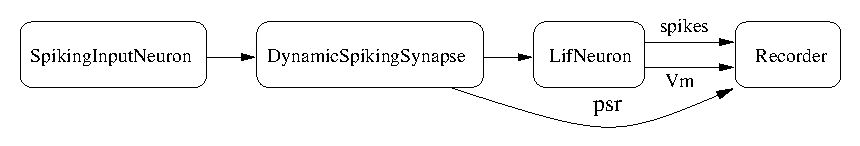
\includegraphics{first-model-csim}
\end{center}

\subsection{Setting up the input} Before we are ready to run the
simulation we have to define the spike train which should be emitted
 by the input neuron \texttt{i}. In \csim time varying
 \secref{sec:inputs}{\emph{input signals}} (analog or spiking) -- also
 called the \emph{stimulus} -- are not considered to be
 properties/attributes of some objects but are always explicitly
 specified. In the case of our example we will define a spike train
 with randomly drawn spike times (for details see \sect{sec:inputs}):
\begin{tabbing}
\quad\tt>> S.spiking = 1;                \% 1 ... spike times, 0 ... analog data\\
\quad\tt>> S.dt      = NaN;              \% resolution for analog data \\
\quad\tt>> S.idx     = i;                \% index/handle of receiving object\\
\quad\tt>> S.data    = sort(rand(1,10)); \% 10 random spikes in the interval 0 to 1 sec
\end{tabbing}

\subsection{Running the simulation} Now we are ready to run the
simulation. The command
%
\begin{tabbing}
\quad\tt>> Tsim=1; \\
\quad\tt>> csim('\hyperlink{cmd:simulate}{simulate}',Tsim,S);
\end{tabbing}
%
simulates the simple model for 1\,sec starting at time
$t=0$\footnote{In general the simulation will be continued at the time
where the last \secref{cmd:simulate}{simulate command}
stopped. However the first simulate command -- as in the case of the
example -- starts at time $t=0$. Simulation time can be reset to time
$t=0$ with the \secref{cmd:reset}{reset command}
\texttt{csim('reset');}.} with the stimulus \texttt{S}.

\subsection{Plotting the recorded traces} The traces recorded by the
recorder can be obtained by the command
\begin{tabbing}
\quad\tt>> t=csim('\hyperlink{cmd:get}{get}',r,'traces')
\end{tabbing}
which yields the output
\begin{verbatim}
t = 
    channel: [1x3 struct]
\end{verbatim}
A closer look at e.g. the first channel reveals that
\texttt{t.channel} is a struct array with a similar structure as we
have seen above for the input signal:
\begin{verbatim}
>> t.channel(1)           

ans = 

          idx: 1
    fieldName: 'psr'
         data: [1x2000 double]
      spiking: 0
           dt: 5.0000e-04
\end{verbatim}

The output indicates that \texttt{t.channel(1).data} holds the
\texttt{psr} trace (\texttt{t.channel(1).fieldName}) with a resolution
of 0.5\,ms (\texttt{t.channel(1).dt}). See the
\secref{classRecorder}{Recorder class documentation} for details abput
the structure of the trace output. Similarly \texttt{t.channel(2)}
holds the the \texttt{Vm} trace and \texttt{t.channel(3)} holds the
output spike times. Hence the following command will plot
the \texttt{psr} trace
\begin{tabbing}
\quad\tt>> plot(t.channel(1).dt:t.channel(1).dt:Tsim,t.channel(1).data);
\end{tabbing}
and the command
\begin{tabbing}
\quad\tt>> stem(t.channel(3).data,ones(size(t.channel(3).data)));
\end{tabbing}
will draw the output spike train.

Using another set of plot commands one can easily create the following
figure which shows the input, the postsynaptic response and the output
of the neuron (the voltage and the spikes)

\begin{center}
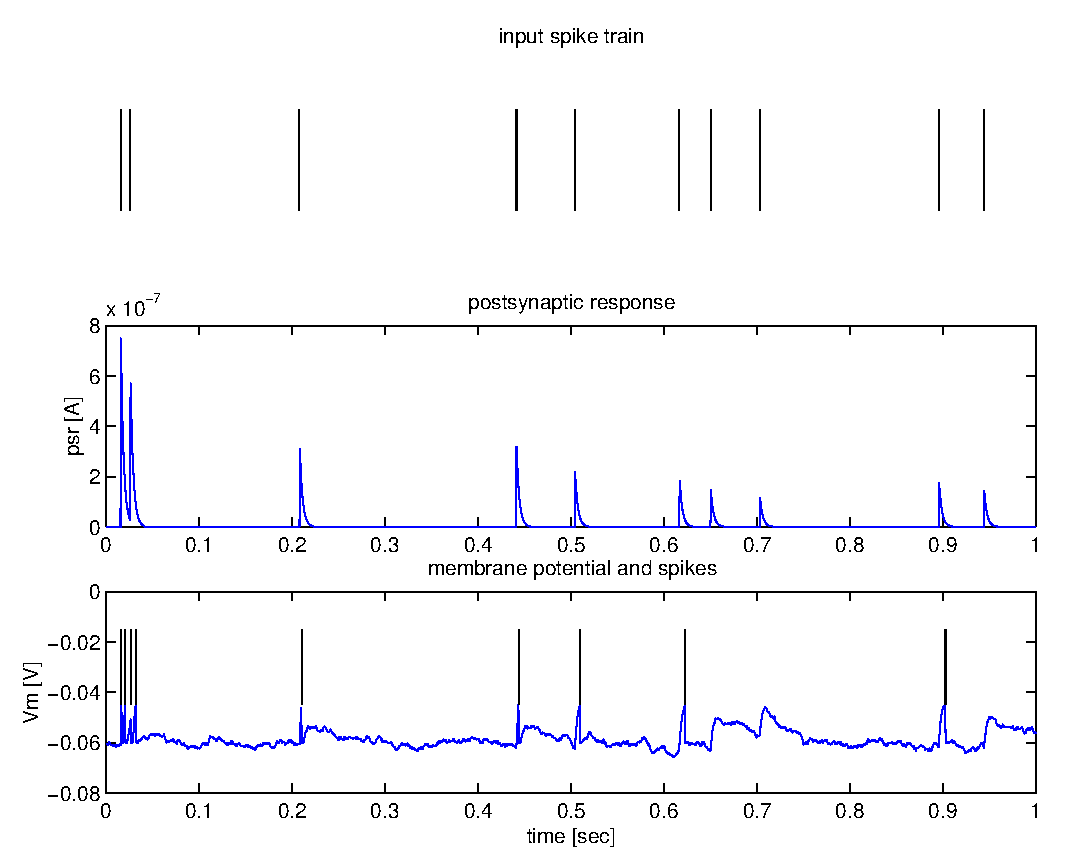
\includegraphics[width=12cm]{first-model-output}
\end{center}

The full code of this example is contained as the file
\texttt{first\_model.m} in the demo directory of the
\href{http://www.lsm.tugraz.at/csim}{\csim package}.


